%!TEX root = ../template.tex
%%%%%%%%%%%%%%%%%%%%%%%%%%%%%%%%%%%%%%%%%%%%%%%%%%%%%%%%%%%%%%%%%%%%
%% chapter4.tex
%% NOVA thesis document file
%%
%% Chapter with lots of dummy text
%%%%%%%%%%%%%%%%%%%%%%%%%%%%%%%%%%%%%%%%%%%%%%%%%%%%%%%%%%%%%%%%%%%%

\typeout{NT FILE chapter4.tex}%

\chapter{Data Description and Management}
\label{cha:data}

\begin{figure}
\centering
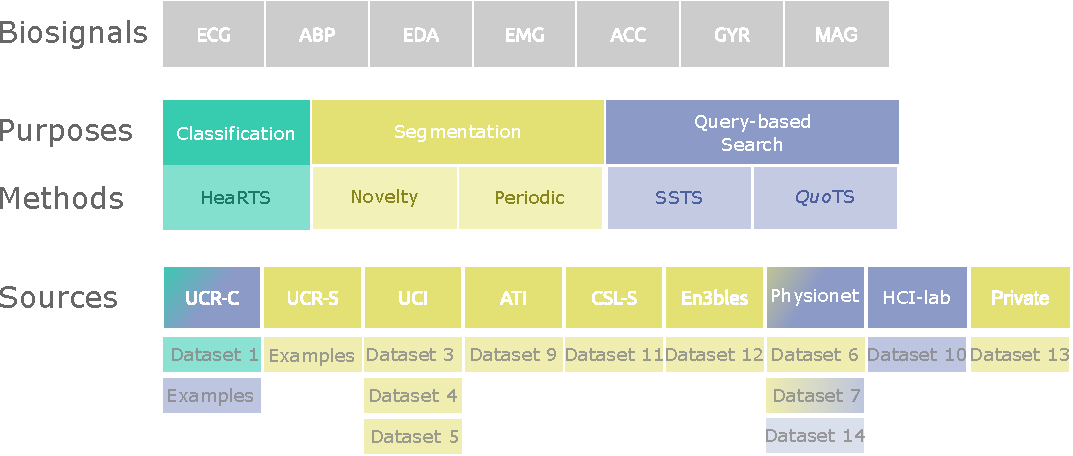
\includegraphics[width=\linewidth]{datasets_intro.pdf}
\caption{Summary of the data used in this work. All types of biosignals where the methods developed in this work were applied to are listed. The three main purposes of the methods developed are presented and color-coded to highlight on each data source which methods were used. \textit{UCR-C}: University California Riverside, and \textit{C} stands for classification; \textit{UCR-S}: \textit{S} stands for segmentation; \textit{UCI}: University California Irvine; \textit{ATI:} Alan Turing Institute; \textit{CSL-S:} Cognitive Systems Lab, where \textit{S} stands for \textit{share}; \textit{HCI-lab:} Human Computer Interaction lab. The tag \textit{Examples} means that several signals were used to demonstrate the usage of the methods as an example. The private source corresponds to the dataset recorded at \textit{Volkswagen Autoeuropa}.}
\label{fig:intro_datasets}
\end{figure}

In this work, we applied the proposed methodologies in a variety of publicly available datasets. Some datasets were used to exemplify how a proposed method could be valuable, in other cases, the datasets were used for validation. The methods developed and presented in this work are agnostic to the type of time series, but we focus all of the examples in \textit{biosignals} data in order to demonstrate the applicability of such methods in the biomedical domain. In addition, most of the \textit{biosignals} used are very common to be acquired in occupational scenarios. Most validations were performed with benchmark datasets, commonly used by the data science community for the tasks approached in this work, and have comparable measures from other existing methods.

Considering the diversity of topics covered, methods developed and datasets used, we summarized the information in Figure \ref{fig:intro_datasets}. We show the types of \textit{biosignals} that were used, the main sources for the publicly available data, and which their purpose in this work. From public datasets we used \gls{ecg}, \gls{abp}, \gls{emg}, \gls{scr}, \gls{acc} and \gls{gyro} biosignals. The purposes of these datasets involved mainly three tasks in the time series data mining domain: classification, segmentation and query-based search. We highlighted the colors corresponding to the purpose that the dataset would be use for. 

A short description of each dataset is provided in this Section, highlighting their purpose in this work. In case an illustration of the signal is not provided during the explanation of the methods' or results' sections, we show an illustrative example of the signal to accompany the description of the dataset.

\section{Datasets}
\label{sec:dataset}

\subsection{Dataset 1 - UCR Classification Benchmark}
\label{sec:dat_ucr}
\textbf{Description}\hfill\\
The University of California Riverside (UCR) Time Series Archive was introduced in 2002 and is one of the most used benchmarks for time series data mining tasks, specially for classification. The datasets are diverse in terms of data type, data domain, difficulty, number of classes and dimensionality\cite{ucr}. Several \textit{python} distributions make it available to download. In this thesis, all UCR archive datasets from the \textit{pyts} distribution were used for classification tasks. These represent 107 datasets from 18 different data types (audio, devices, \gls{ecg}, \gls{eog}, \gls{eeg}, \gls{har}, etc...), which also are from many different domains, such as medical, financial, motion, entomology, etc...\cite{ucr}. The list of datasets can be found on the following link \cite{ucr_site} and in Appendix \ref{app:datasets}.\\
\textbf{Purpose}\hfill\\
The UCR-C dataset is the benchmark used to validate \gls{hearts} for the classification task. Several signals from this dataset are used as examples as well to demonstrate the usage of \gls{quots} in query-based search tasks.\\
\textbf{Ground Truth}\hfill\\
The benchmark has a guideline in how to use it correctly at \cite{ucr}. It has a pre-defined training and testing set. In case parameters have to by estimated during the training stage, it is recommended to use a cross-validation on the training set. In this work, these guidelines were followed to validate \gls{hearts}.

\subsection{Dataset 2 - Physiological Response to Changes in Posture}
\label{dat:dataset2}

\textbf{Description}\hfill\\
In the dataset \cite{tilt}, ten subjects' slow tilt, rapid tilt and standing-up activities were monitored and recorded with \gls{ecg} and \gls{abp} to investigate how the two physiological signals respond to the angular changes during the mentioned activities \cite{tilt, PhysioNet}.\\
\textbf{Purpose}\hfill\\
The dataset's \gls{abp} channel was used as an example to demonstrate the usage of the \gls{ssm}'s novelty function in detecting pattern-based physiological changes in a distinctive research instance.\\
\textbf{Ground Truth}\hfill\\
The ground truth of the changes is marked by the angular signal, suggesting the moments a tilt or standing up activity occurred. The angular signal can have different shapes (rectangular or trapezoid), which depends on the speed at which the posture changes.
 
\subsection{Dataset 3 - Smartphone Dataset for Human Activity Recognition in Ambient Assisted Living}
\label{dat:dataset3}

\begin{figure}
\centering
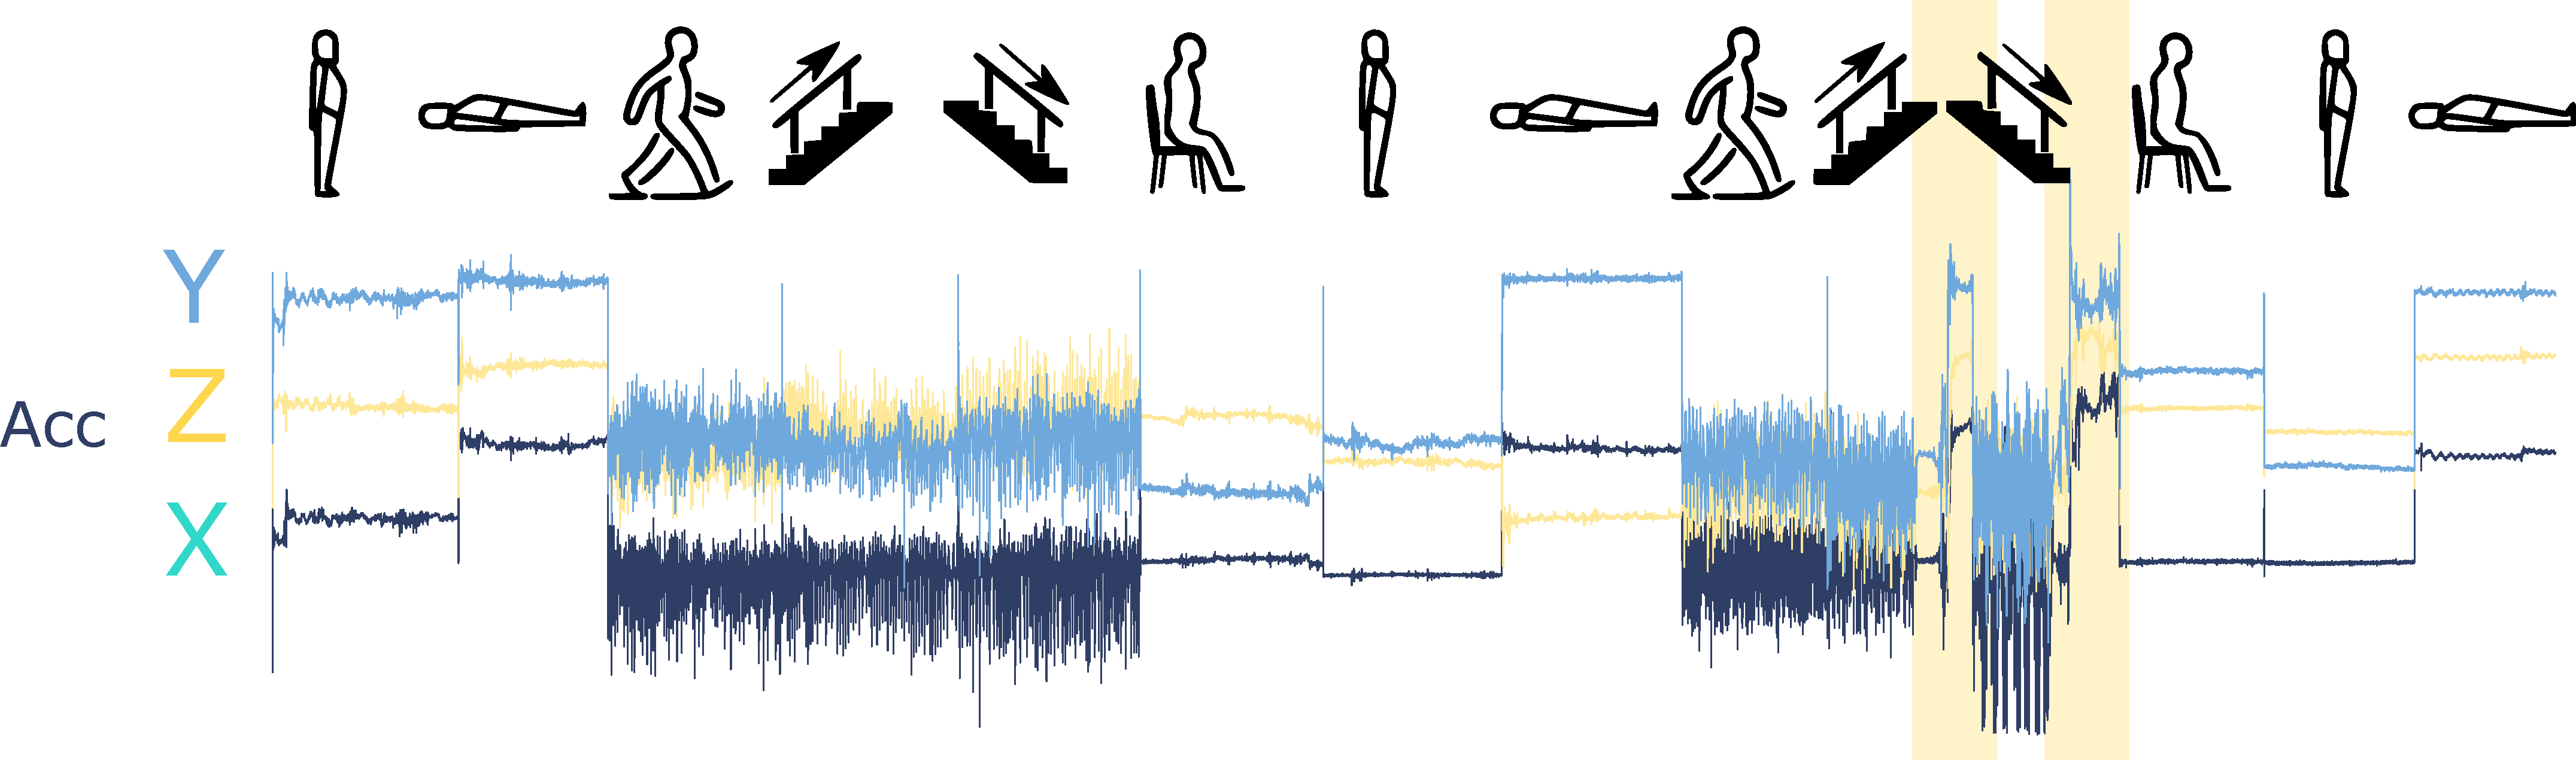
\includegraphics[width=\linewidth]{datasets/har_2_dataset.pdf}
\caption{Example of the signal for this dataset. It shows the 3 axis of the accelerometer signal and the corresponding labels in each section \cite{dataset2, dataset2_2}. Yellow areas indicate moments where there was a change on the signal not related with the labeled activity.}
\label{fig:har2_dataset}
\end{figure}

\textbf{Description}\hfill\\
This dataset was gathered from an experiment on 30 volunteers. Each subject was wearing a smartphone on the waist while performing several activities: \textit{(1) Walking, (2) Walking Upstairs, (3) Walking Downstairs, (4) Sitting, (5) Standing and (6) Laying}. The activities were performed for approximately 60 seconds. The device recorded the internal \gls{acc} and \gls{gyro} data at a constant rate of 50 Hz. Each activity has been categorized and labeled on the acquired data \cite{dataset2, dataset2_2}.\\
\textbf{Purpose}\hfill\\
This dataset was used in the context of novelty segmentation \cite{dataset2, dataset2_2}.\\
\textbf{Ground Truth}\hfill\\
Each file has a ground-truth signal that can be used to validate the novelty segmentation approach with the \gls{ssm}'s novelty function. A specific value is attributed to each class, which changes continuously over time and is aligned with the signal. The transitions between these activities are kept as the reference events for the validation.
    
%\subsection{Dataset 4 - Smartphone-Based Recognition of Human Activities and Postural Transitions}
%\label{dat:dataset4}
%\textbf{Description}\hfill\\
%The dataset was built in the context of human activity recognition experiments. These were carried out with a group of 30 volunteers that performed a protocol with six basic activities: three static postures (standing, sitting, lying) and three dynamic activities (walking, walking downstairs and walking upstairs). Additionally, the experiment also included postural transitions that occurred between the static postures. These are: stand-to-sit, sit-to-stand, sit-to-lie, lie-to-sit, stand-to-lie, and lie-to-stand. The data was collected with a smartphone (Samsung Galaxy S II) mounted on the waist of each subject. The data from a 3-axis accelerometer and 3-axis gyroscope was gathered at a constant rate of 50Hz. The experiments were video-recorded to label the data manually \cite{dataset3}.\\
%\textbf{Purpose}\hfill\\
%This dataset was used in the context of novelty segmentation \cite{dataset3}.
%
%\begin{figure}
%\centering
%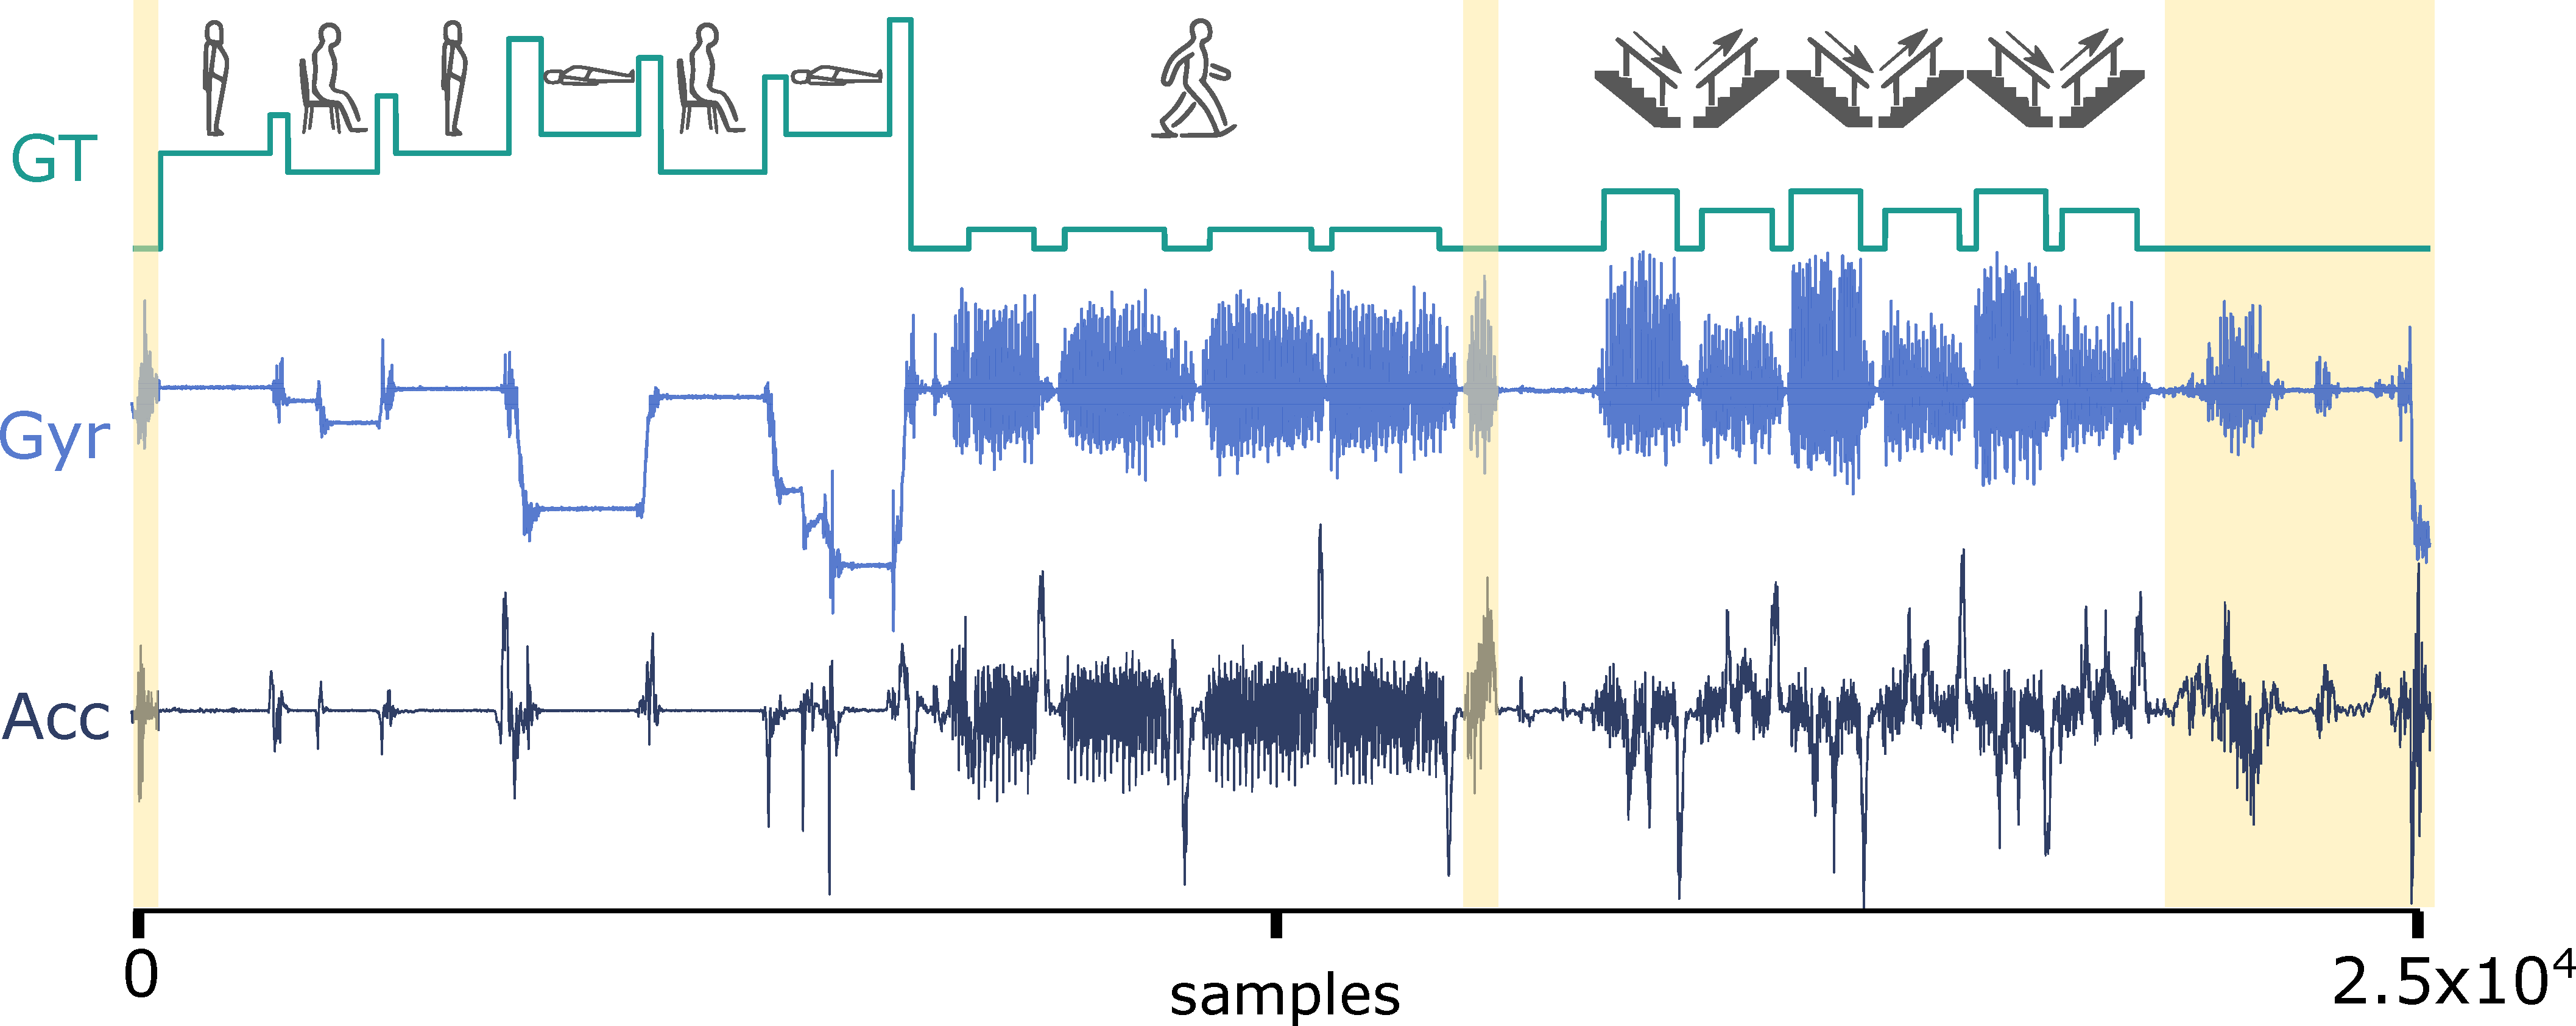
\includegraphics[width=\linewidth]{datasets/har_1_dataset.pdf}
%\caption{Example of the signal for this dataset. It shows one axis for the \gls{acc} and \gls{gyro} signals and the corresponding labels in each section \cite{dataset3}. In this datasets, labels also highlight posture transitions, such as \textit{Standing to Sitting}. Yellow areas indicate moments where there is activity but the signal was not labeled.}
%\label{fig:har1_dataset}
%\end{figure}    
    
\subsection{Dataset 4 - Wireless Sensor Data Mining (WISDM) Smarphone and Smartwatch Activity Biometrics Dataset}
\label{dat:dataset5}

\begin{figure}
\centering
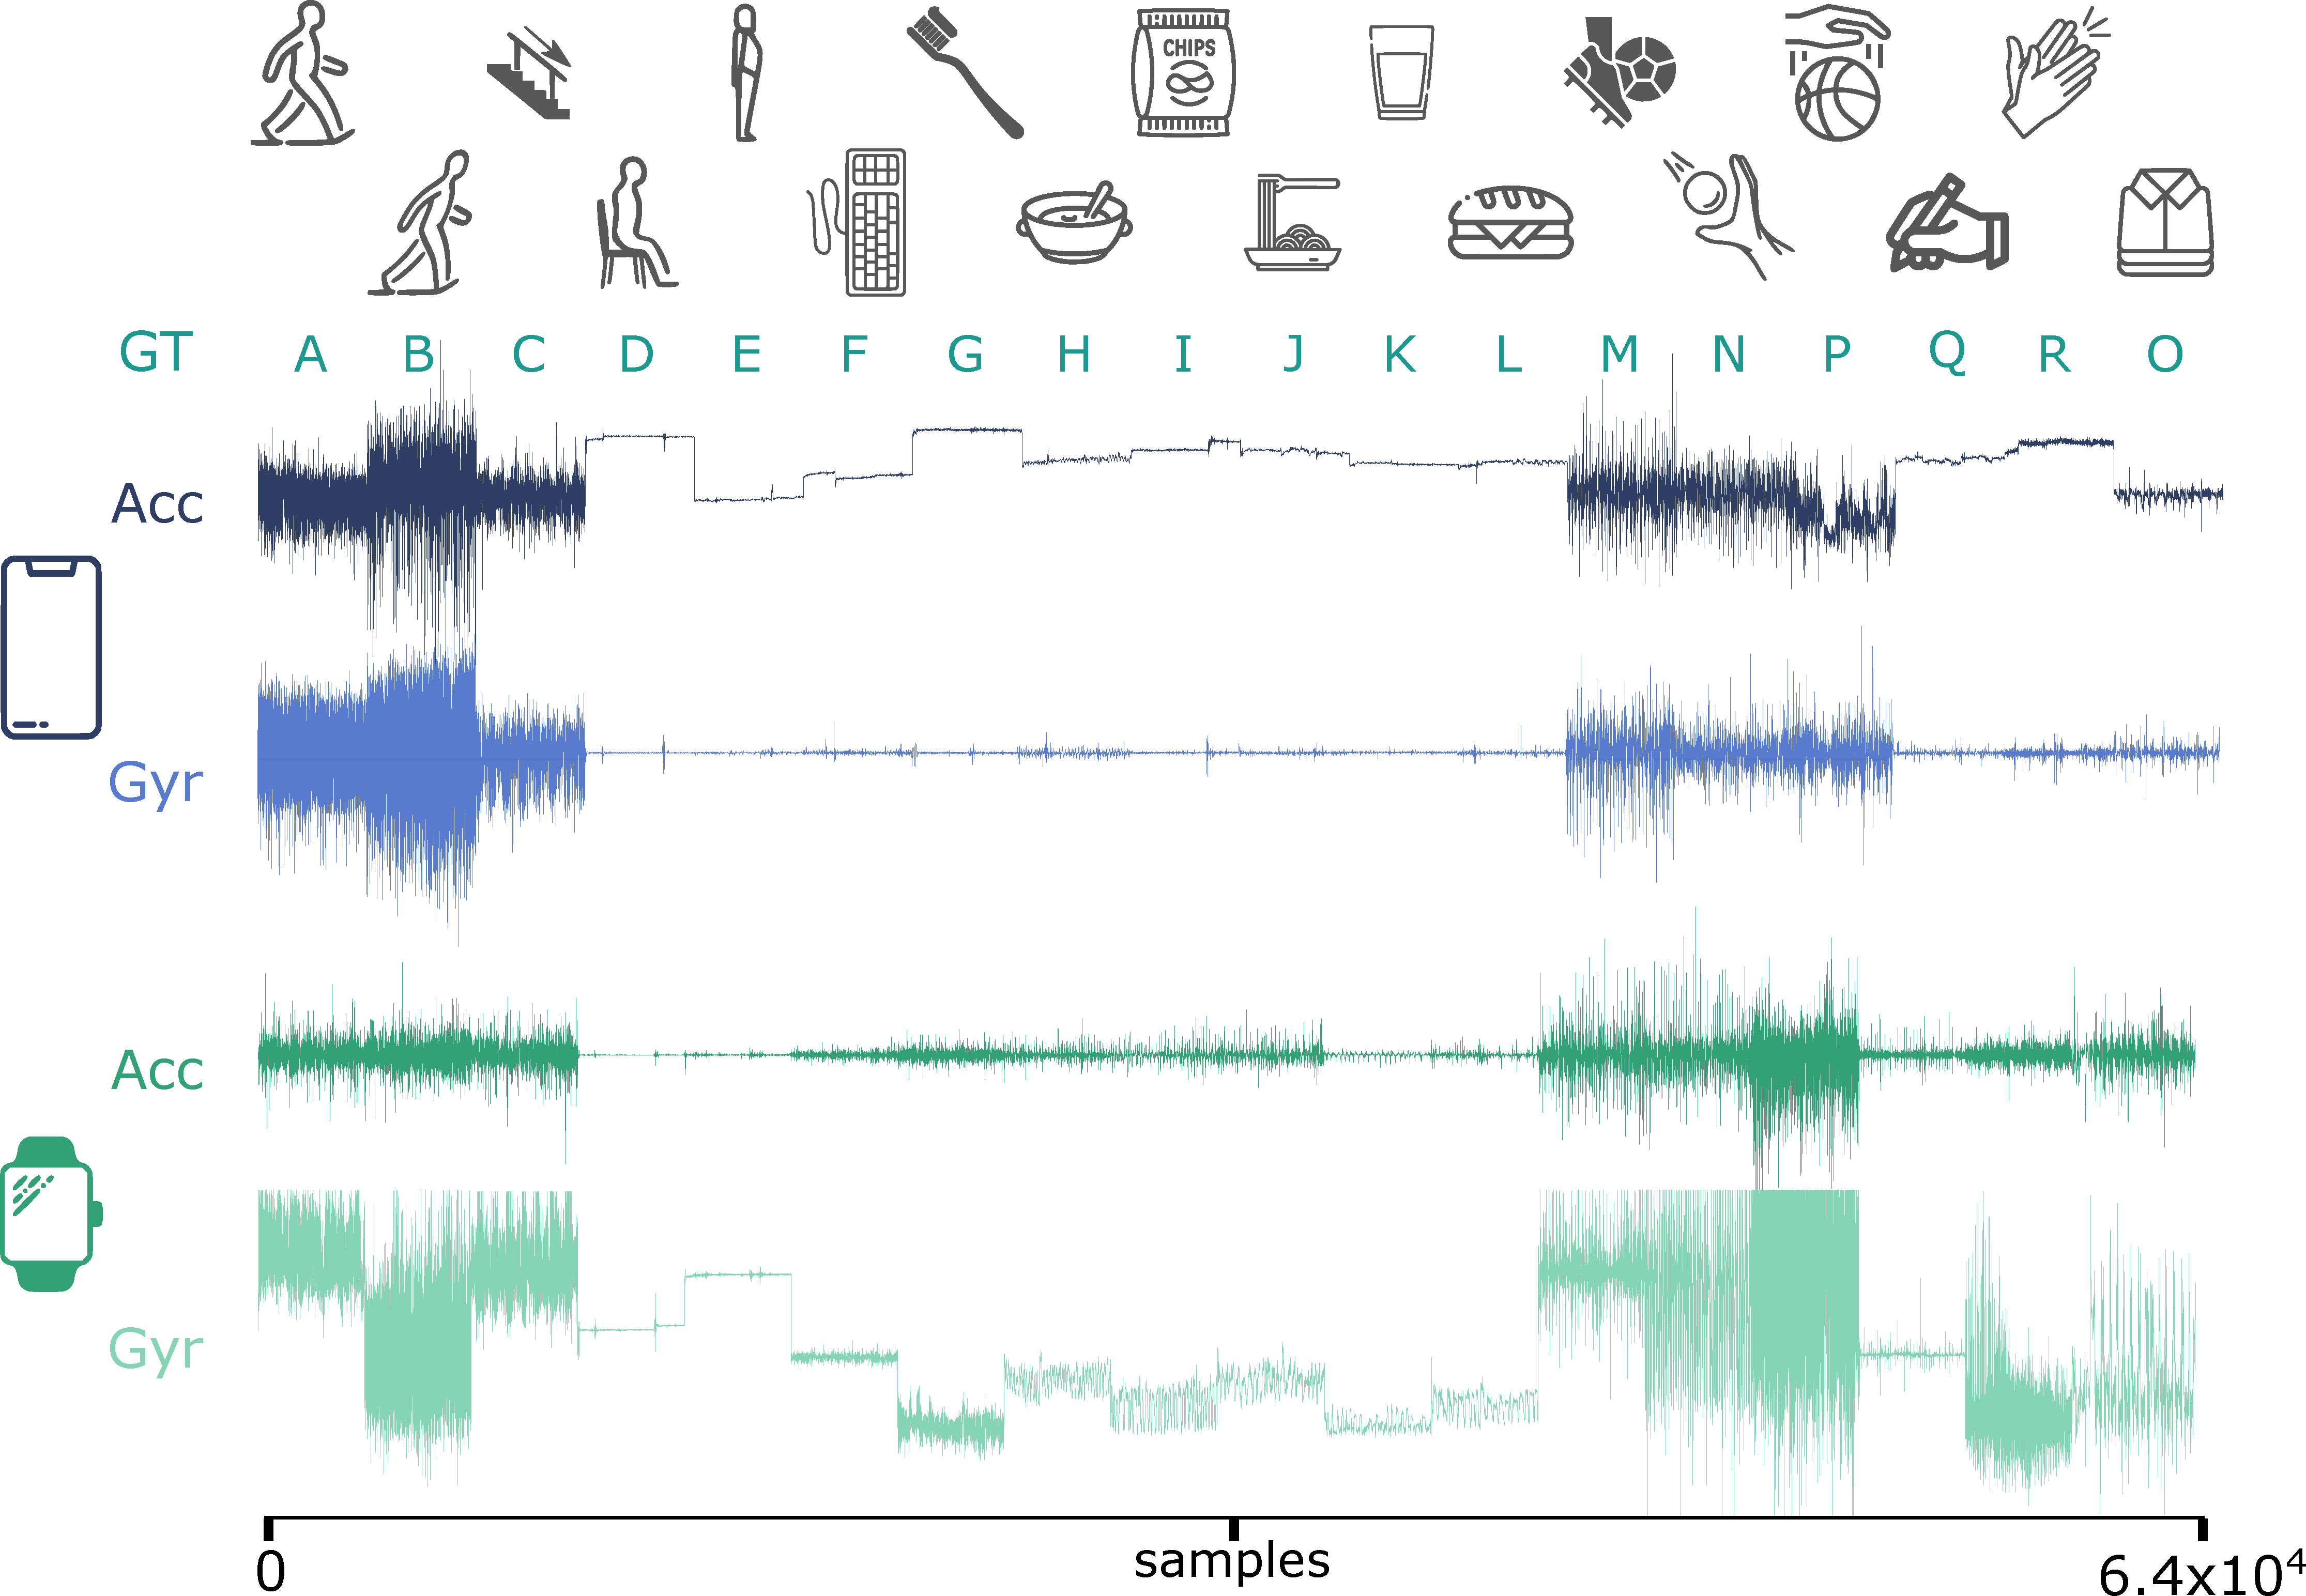
\includegraphics[width=\linewidth]{datasets/wisdim_dataset.pdf}
\caption{Example of the signal for this dataset. It shows one axis of each type of data acquired, for both smartphone and smartwatch. The activities are highlighted as well and labeled as: A - walking, B - running, C - walking on stairs, D - sitting, E - standing, F -   typing, G - brushing, H - eating soup, I - eating chips, J - eating pasta, K - drinking, L - eating a sandwich, M - kicking, N - catching a ball, P - dribbling, Q - writing, R - clapping, O - iron \cite{dataset4}.}
\label{fig:wisdim_data}
\end{figure}

\textbf{Description}\hfill\\
The raw data from the accelerometer and gyroscope sensors is collected from a smartphone and smartwatch at a rate of 20Hz. This experiment was conducted on 51 participants as they performed 18 activities, each for a duration of 3 minutes. Each sample of the data was labelled based on the activity it corresponds to. The activities are diverse and include dribbling, eating, jogging, sitting, walking on stairs, standing, walking, among others \cite{dataset4}. Figure \ref{fig:wisdim_data} illustrates an example of this type of data.\\
\textbf{Purpose}\hfill\\
This dataset was used in the context of novelty segmentation in complex real-life scenarios.\\
\textbf{Ground Truth}\\
The ground truth is available for each file and each activity. For the task of novelty search, we used the transition between labels as the reference instant of a change, as we did with the previous dataset.

\subsection{Dataset 5 - EMG Data for Gestures}
\label{dat:dataset6}

\begin{figure}
\centering
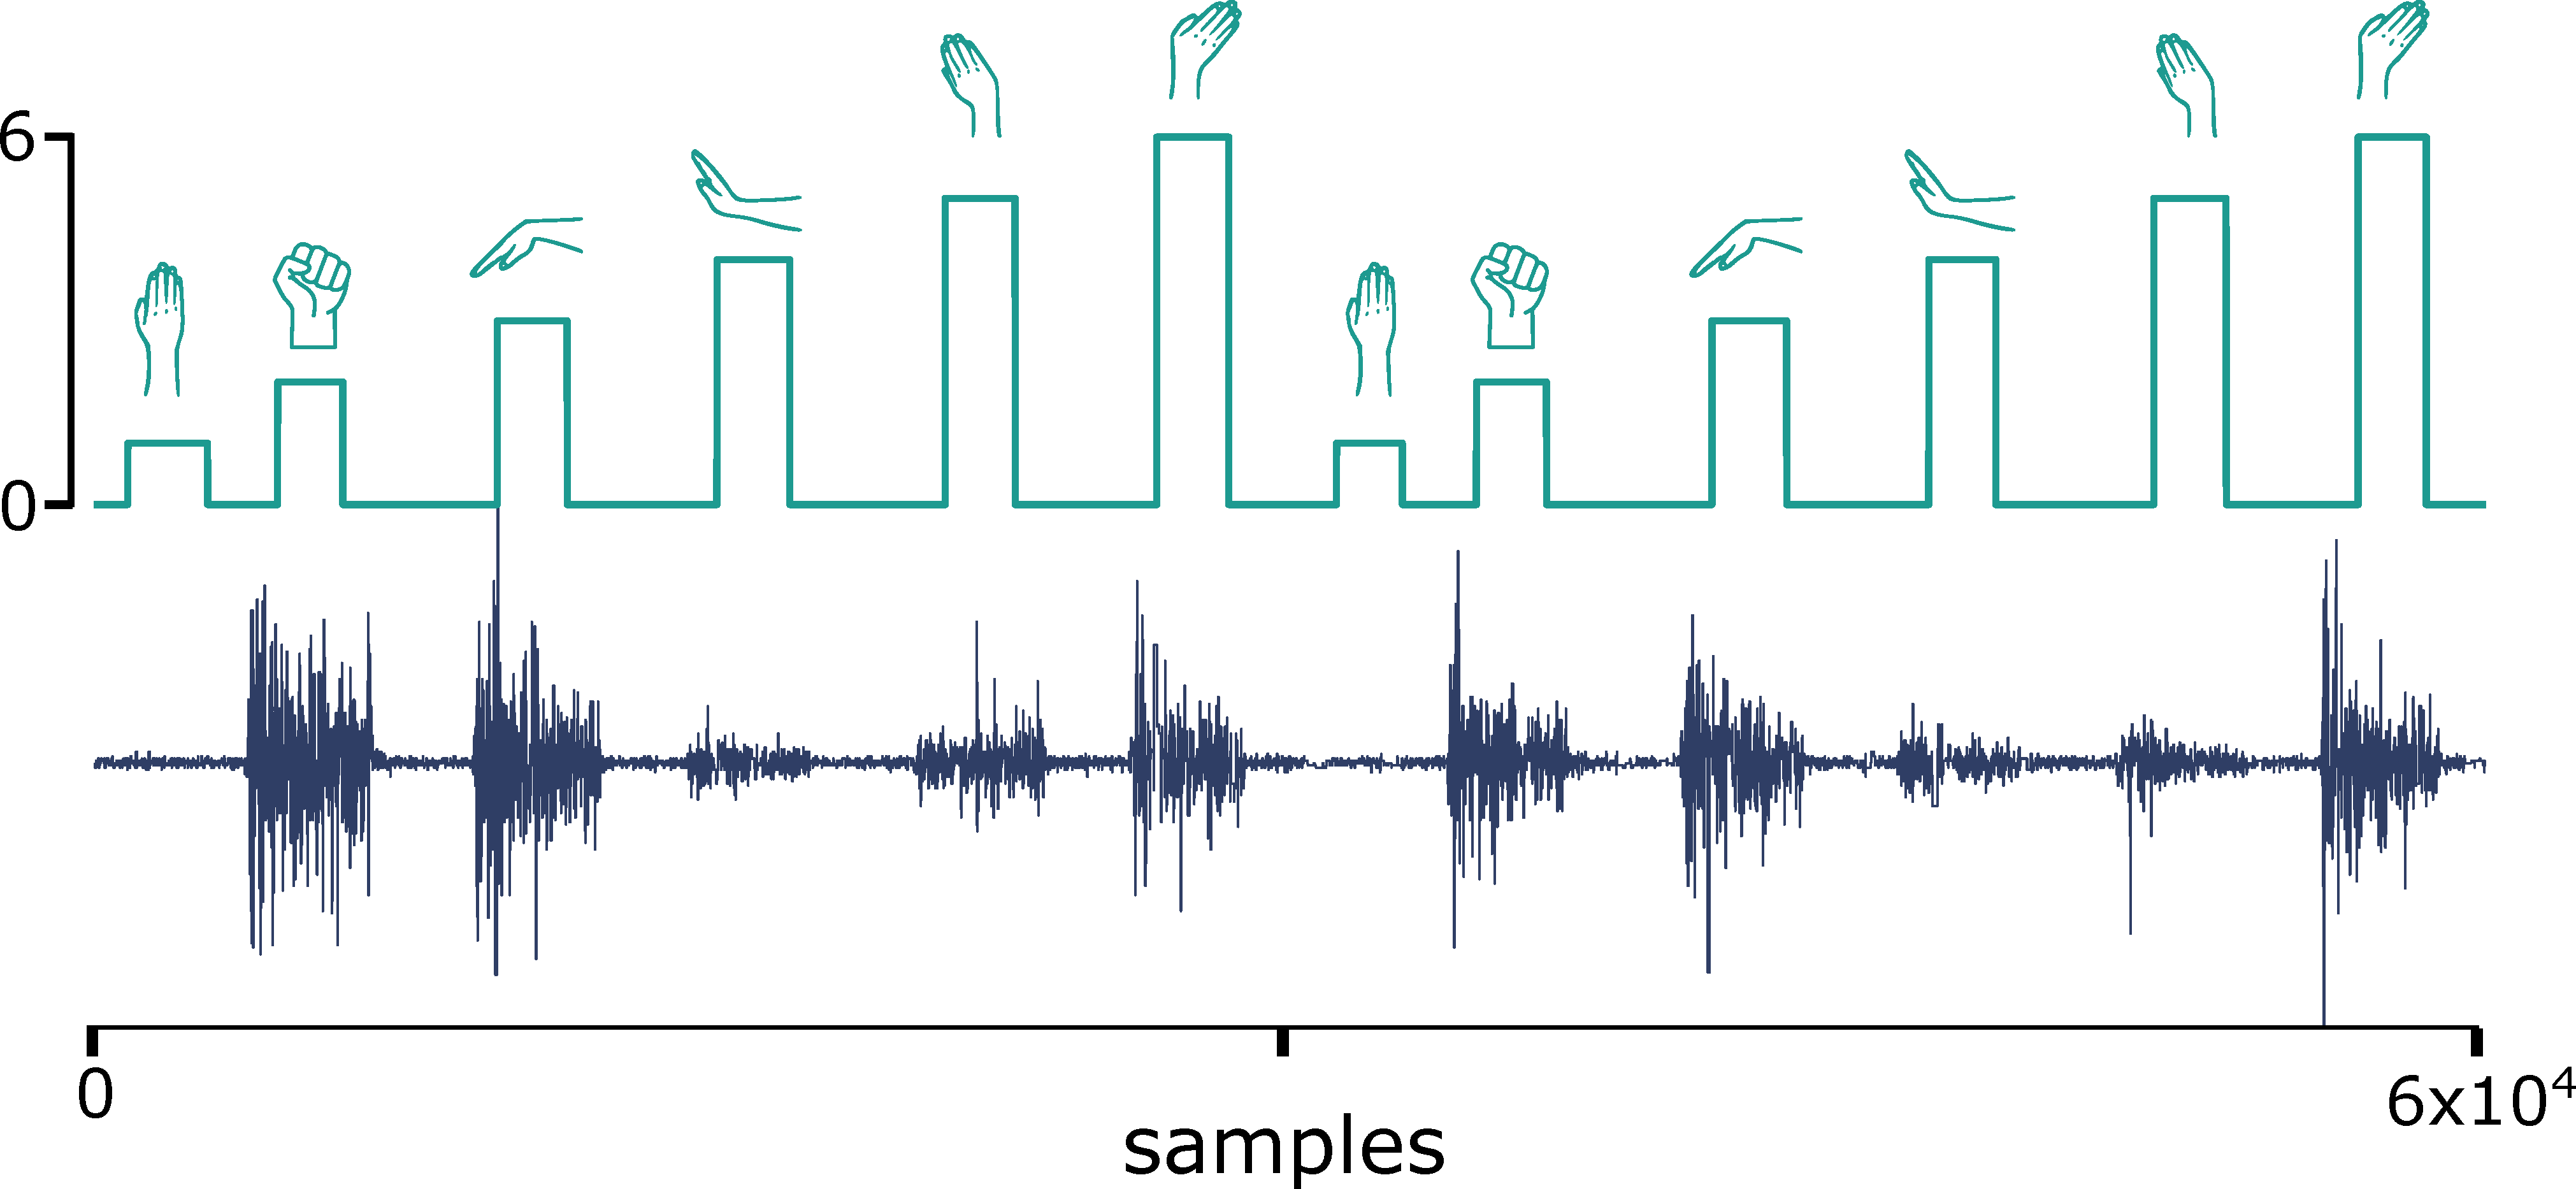
\includegraphics[width=\linewidth]{datasets/emg_dataset.pdf}
\caption{Example of the \gls{emg} data and the corresponding hand postures.}
\label{fig:emg_dataset}
\end{figure}

\textbf{Description}\hfill\\
This dataset has EMG signals for recording patterns, by using a MYO Thalmic bracelet worn on a user's forearm. The bracelet is equipped with eight sensors equally spaced around the forearm that simultaneously acquire electromyographic signals. The dataset has raw EMG data from 36 subjects while they performed series of static hand gestures. The subject performs two series, each of which consists of six basic gestures. Each gesture was performed for 3 seconds with a pause of 3 seconds between gestures. The data was collected with a fixed sampling frequency of 200 Hz \cite{dataset5}.\\
\textbf{Purpose}\hfill\\
This dataset was used in the context of novelty segmentation, to test the method in estimating transitions between the activation (onset) and relaxation (offset) of the muscular activity.\\
\textbf{Ground Truth}\\
The ground truth is available for each file and each activity. For the task of novelty search, we used the transition between labels as the reference instant of a change. As indicated in Figure \ref{fig:emg_dataset}, the ground truth would have considered as events the absence of activity (which the original dataset uses because it was designed for a classification problem). In this case, we did not considered these events in our ground truth for this dataset for the problem of segmentation.    

\subsection{Dataset 6 - MIT-BIH Noise Stress Test Database}
\label{dat:dataset7}

\begin{figure}
\centering
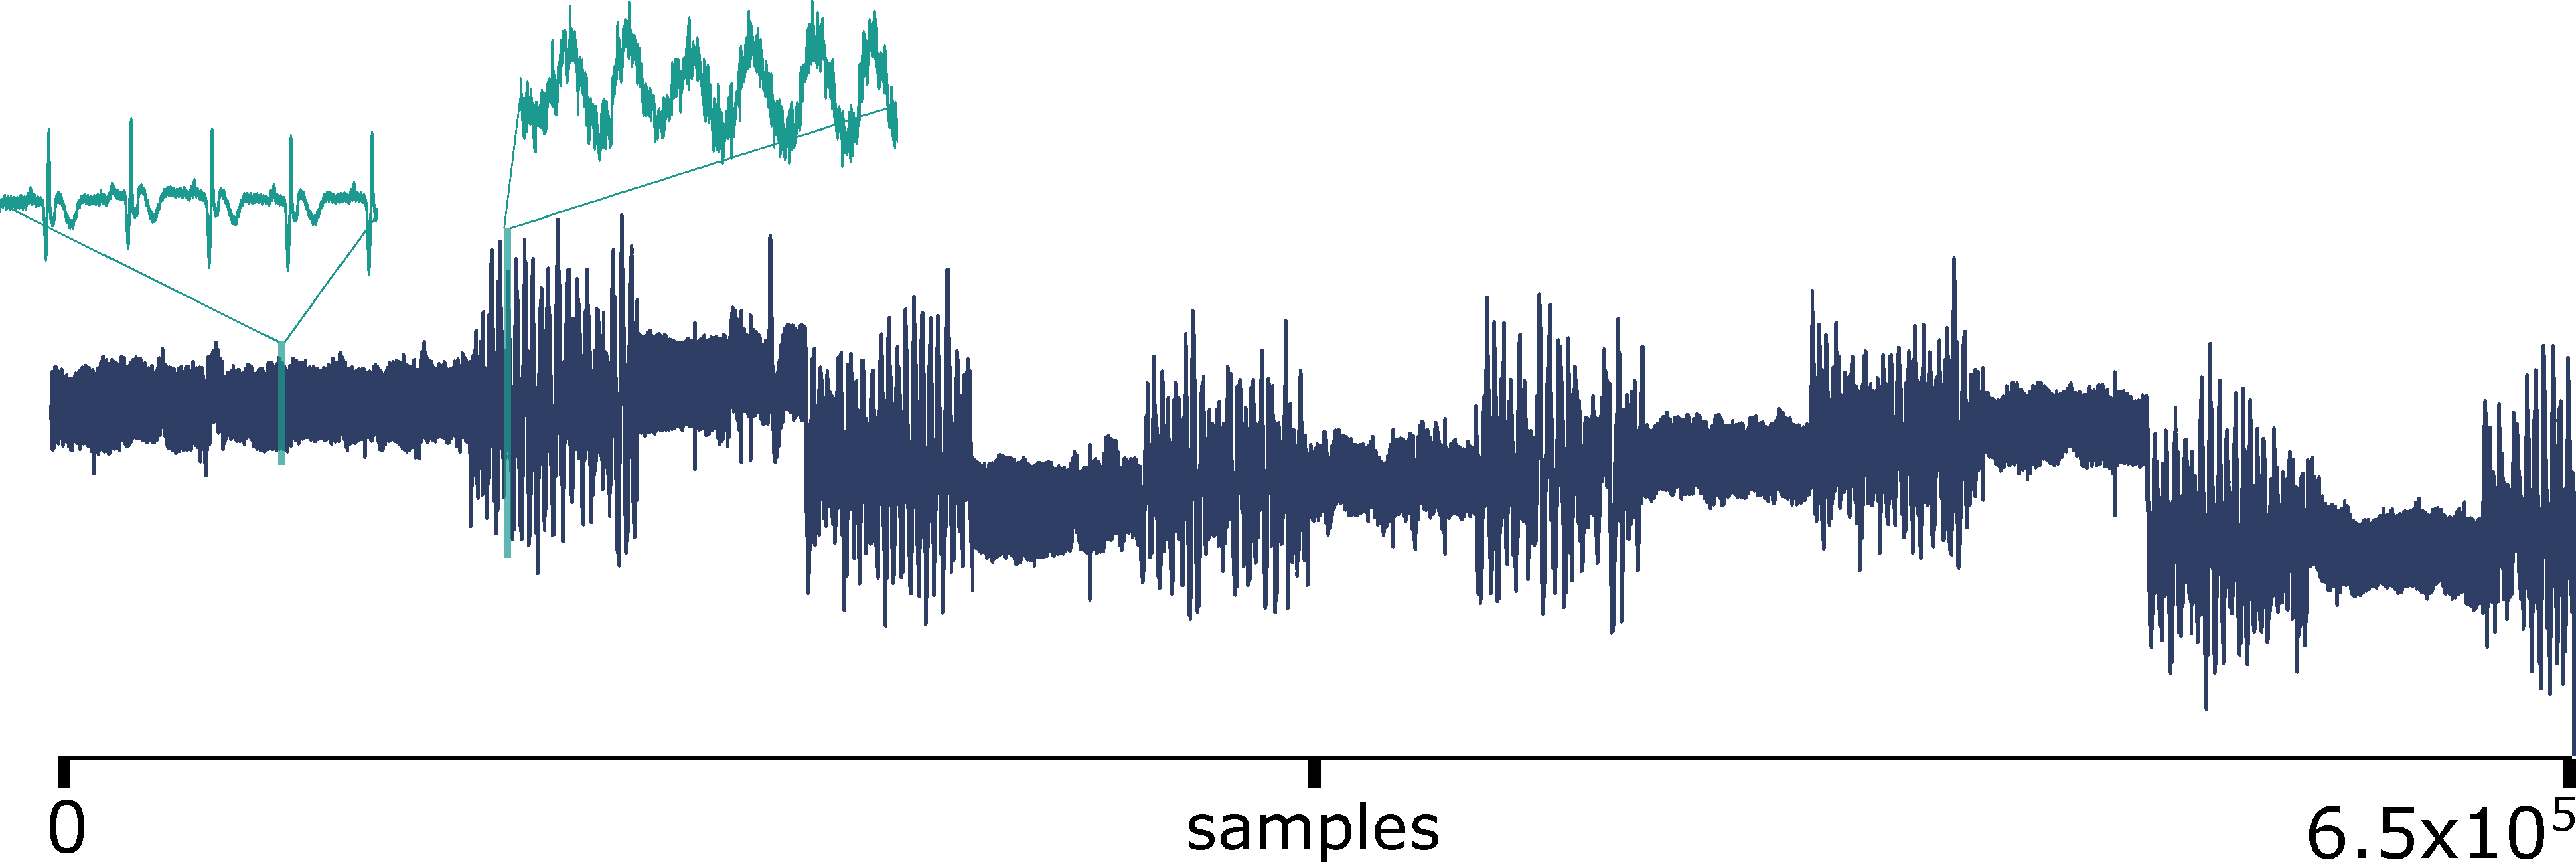
\includegraphics[width=\linewidth]{datasets/ecg_noise1.pdf}
\caption{Example of an \gls{ecg} record contaminated with noise. Two sections are highlighted showing the clean and contaminated area of the signal. \cite{dataset7}}
\label{fig:ecg1_dataset}
\end{figure}

\textbf{Description}\hfill\\
The dataset comprehends 12 half-hour \gls{ecg} recordings and 3 half-hour recordings of noise typical in ambulatory \gls{ecg} recordings. The noise recordings were made using physically active volunteers and standard \gls{ecg} recorders, leads, and electrodes. The three noise records were assembled from the recordings by selecting intervals that contained predominantly baseline wander (in record 'bw'), muscle (EMG) artifact (in record 'ma'), and electrode motion artifact (in record 'em'). Two clean \gls{ecg} signals were selected and noise was added with different signal-to-noise ratios (SNR) \cite{dataset6, PhysioNet}.\\
\textbf{Purpose}\hfill\\
This dataset was used in the context of novelty segmentation, to test the method in estimating transitions to and from noise sections of the signal.\\
\textbf{Ground Truth}\\
The reference events were manually annotated based on the signal with lower \gls{snr}. All noise presence is located in the same regions of the signal, only with different \gls{snr}.

    
\subsection{Dataset 7 - Motion Artifacted Contaminated \gls{ecg}}
\label{dat:dataset8}
\begin{figure}
\centering
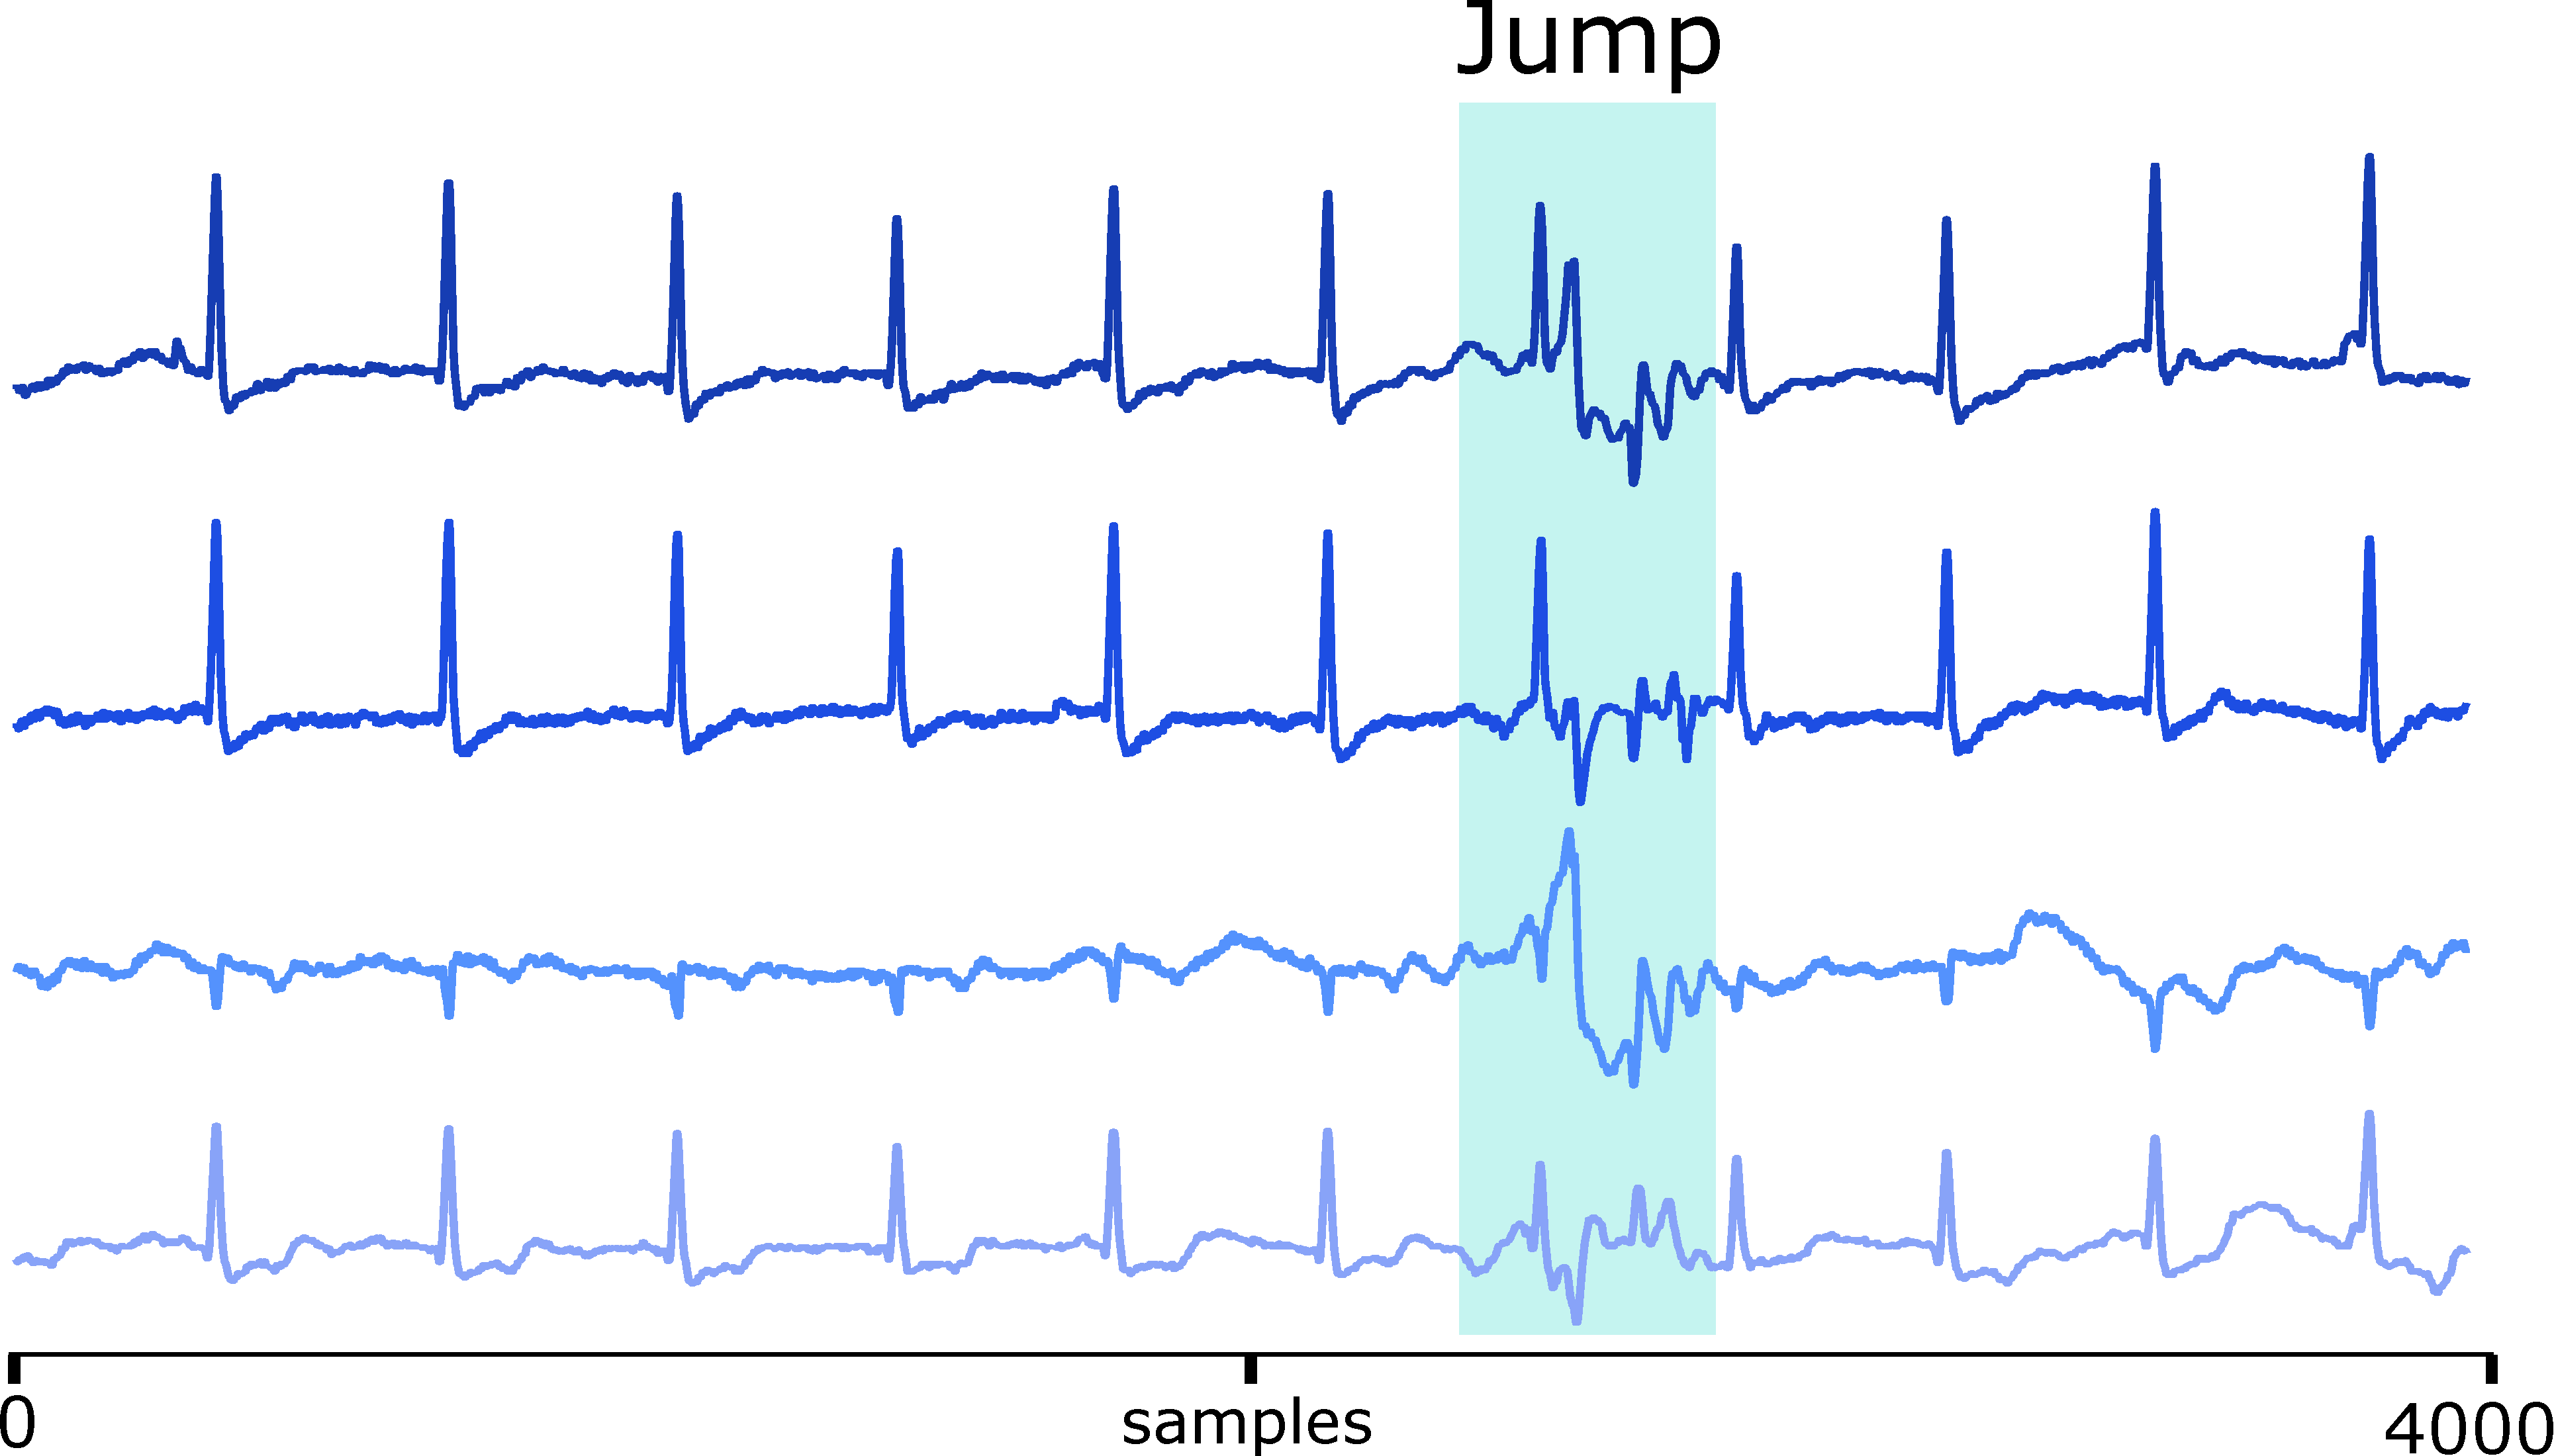
\includegraphics[width=0.85\linewidth]{datasets/ecg_noise2.pdf}
\caption{Example of an \gls{ecg} signal contaminated with motion artifacts. The artifact is visible due to a jump from the subject.}
\label{fig:ecg2_dataset}
\end{figure}

\textbf{Description}\hfill\\
This dataset has short duration \gls{ecg} signals, which were recorded from a healthy 25-year-old male performing different physical activities (standing, walking and single jump) to study the effect of motion artifacts on \gls{ecg} signals and their sparsity. The dataset was acquired with a sampling rate of 500 Hz and 16 bit resolution. For this exercise, only the records with jump were used \cite{dataset7, PhysioNet}.\\
\textbf{Purpose}\hfill\\
This dataset was used in the context of change point detection, to test the method in estimating transitions to and from noise sections of the signal.\\
\textbf{Ground Truth}\\
The reference events were manually annotated in the intervals of noise due to a jump activity.

%\section{Dataset 5 — Arterial Blood Pressure}
%\label{dat:abp}
%
%\textbf{Description}\hfill \\ 
%In the dataset \cite{tilt}, ten subjects' slow tilt, rapid tilt and standing-up activities were monitored and recorded with \gls{ecg} and \gls{abp} to investigate how the two physiological signals respond to the angular changes during the activities\cite{tilt, physionet}.\\
%\textbf{Purpose} \hfill\\
%The dataset's \gls{abp} channel was used as an example to demonstrate the proposed algorithm's capability in detecting pattern-based physiological changes in a distinctive research instance.\\
%\textbf{Ground Truth}\hfill \\
%
%The ground truth of the changes is marked by the angular signal, suggesting the moments a tilt or standing up activity occurred.

\subsection{Dataset 8 - St Petersburg INCART 12-lead Arrhythmia Database}
\label{dat:dataset9}
\textbf{Description}\hfill \\
This dataset has \gls{ecg} signals from patients undergoing tests for coronary artery disease. 75 annotated recordings were extracted. Each record is 30 minutes long and has 12 leads, each sampled at 257 Hz. The annotations include beats as well as relevant artifacts/occurrences present on the signal, such as arrhythmia \cite{PhysioNet}. Records \textit{I02, I04 and I09} were used.\\
\textbf{Purpose}\hfill \\
This dataset was used in the context of pattern search with \gls{quots} for the detection of different types of arrythmia.\\
\textbf{Ground Truth}\\
The \gls{ecg} beats were detected by an automatic algorithm, which were then manually corrected when needed. The location and type of arrhythmia is available on the dataset \cite{ecg_arrhythmia}.

\subsection{Dataset 9 - Alan Turing CPD Benchmark}
\label{dat:dataset10}
\textbf{Description}\hfill \\
The Alan Turing Change Point Detection Benchmark is a recent dataset used to have a standard reference for change point segmentation tasks. The benchmark was created in 2020 and provides 42 datasets, being 42 univariate time series and 4 multi dimensional time series. The dataset comprises several time series from real-world data. It was built from a project of the Alan Turing Institute to have a repository for the evaluation of change point detection algorithms. The available benchmark page was used to get access to the datasets, and run the performance metrics developed. This way, the performance of the proposed method is compare with the performance of several existing methods \cite{cpd_alan}.\\
\textbf{Purpose}\hfill \\
This dataset has ground-truth events for each time series. The performance of several existing methods is available and used to compare with the performance of the proposed method on the same time series.\\
\textbf{Ground Truth}\\
The signals available in this dataset were manually annotated by several human annotators. Each signal has, in most cases, more than one reference annotation. The evaluation of an algorithm's performance in event detection follows the same metrics as the ones mentioned in \ref{subsec:event_metrics}, but combines the information of multiple annotators \cite{cpd_alan}.

\subsection{Dataset 10 - HCILab Behavioural Driving Dataset}
\label{dat:dataset11}
\textbf{Description}\hfill\\
It is a public dataset that studied ways of assessing the driver's workload combining auto telemetry data with physiological sensors. The authors conducted a real world driving experiment with 10 participants measuring a variety of physiological data as well as a post-hoc video rating session \cite{hcilab}. It includes a variety of physiological signals, such as \gls{ecg} and corresponding heart rate, \gls{scr} and body temperature. In addition, it collected driving speed and GPS location. The map of the driving site can be seen at \cite{hcilab}\\
\textbf{Purpose}\hfill \\
This dataset was used for \gls{quots} in pattern search. For the example presented we used the data of participant number 10 \cite{hcilab}.\\
\textbf{Ground Truth}\hfill \\
The dataset is not originally labelled. In this work, the signals were explored with the \gls{quots} tool to search for relevant patterns that could be associated with relevant occurrences during the driving experience. Although the videos were not available, the GPS data was provided and could be used to match the position of the car with the physiological signals.

\subsection{Dataset 12 - CSL-Share Dataset}
\label{dat:dataset12}
\textbf{Description} \hfill \\
The CSL-SHARE (Cognitive Systems Lab Sensor-based Human Activity REcordings) has twenty two types of activities of daily living and sports recorded in tewnty subjects. It contains multimodal data with two triaxial \gls{acc}, two triaxial \gls{gyro}, four surface \gls{emg} sensors, one biaxial \gls{gonio}, and one airborne microphone integrated into a knee bandage \cite{share}. Seventeen activities were used for this purpose, which were the following: \textit{Sit}, \textit{Sit-to-Stand}, \textit{Stand}, \textit{Stand-to-Sit}, \textit{Stair-Up}, \textit{Stair-Down}, \textit{Walk}, \textit{Curve-Left-Step}, \textit{Curve-Left-Spin}, \textit{Curve-Right-Step}, \textit{Curve-Right-Spin}, \textit{Run}, \textit{V-Cut-Left}, \textit{V-Cut-Right}, \textit{Lateral-Shuffle-Left}, \textit{Lateral-Shuffle-Right}, \textit{Jump-One-Leg}, \textit{Jump-Two-Leg}.\\
\textbf{Purpose}\\
Each activity was performed multiple times in one record. This dataset was used for the onset periodic segmentation of each activity for each record of each subject.\\
\textbf{Ground Truth}\\
A ground-truth squared signal was generated with a push-button during the acquisitions \cite{share}. The transitions between null and positive square wave indicate the onset and offset of the activity of a record. These transitions were used as the ground-truth.

\subsection{Dataset 13 - EN3BLES}
\label{dat:dataset13}
\textbf{Description}\\
The ENABL3S dataset contains bilateral \gls{emg} and motion data from inertial wearable sensors positioned on joints and limbs. Ten subjects participated in the recording, which involved freely transitioning between sitting, standing, and five walking-related activities. In total, 23 sensors were used (14 \gls{emg}, 4 \gls{gonio}, 5 \gls{imu}) and 52 channels (14 \gls{emg}, 8 \gls{gonio}, 30 \gls{imu} - 5 triaxial \gls{acc} + 5 triaxial \gls{gyro}) \cite{enables}.\\
\textbf{Purpose}\\
The dataset was used for the segmentation of activities, made by finding the break-points on the multimodal time series.\\
\textbf{Ground Truth}\\
The labels of each activity were available for each dataset. The segmentation points used as ground truth are the transitions between labels.

\subsection{Dataset 14 - Industrial Job Dataset}
\label{dat:dataset_industry}
\textbf{Description}\hfill \\
A private dataset was acquired at \textit{Volkswagen Autoeuropa} in the context of this thesis, a master thesis from \cite{santos2019} and project \textit{OPERATOR}, in partnership with Fraunhofer AICOS. This dataset used a wearable system with inertial sensors to record direct measures that could be used to calculate the occupational exposure to risk factors of workers during work. The technologycal setting consisted of four 9-\gls{dof} \gls{imu} sensors (composed internally by a triaxial \gls{acc}, triaxial \gls{gyro} and triaxial \gls{mag}) and an Android wireless communication system, which was responsible to record and allocate the data \cite{santos2019}.
\par
The acquisition was made in a \textit{Volkswagen Industrial} assembly line where twelve manufacturing collaborators performed their tasks while having attached the system in their dominant upper body segment (back of hand, wrist, elbow and trunk). The data was recorded in three different workstations from the \textit{Bodyshop assembly line}, which is one section where the cars' doors are assembled. The three workstations are designated: 1) Liftgate workstation, where back doors are mounted; 2) Fender workstation, involving front door tasks and 3) Doors workstation, which demanded tasks on the front doors and in the cars' hood \cite{santos2019}. A total of six operators performed at least two different workstations. All recordings were filmed for posterior visual evaluation. The videos and signals were synchronized by a simultaneous event visible in both video and inertial signals. The event corresponds to a sequence of poses: 1) neutral anatomic position, 2) T pose, 3) return to neutral anatomic position, to finally 4) jump.

The mentioned study was centered on the ergonomic assessment of the dominant arm. For this reason, the \gls{imu}s  were attached in: 1) the posterior side of the hand, 2) posterior side of the forearm and 3) posterior side of the arm and a final one 4) placed in the anterior side of the thorax area. All of the devices were attached with elastic bands, in such a way that all had their Y-axis pointed up while in a neutral anatomical position \cite{sara2019}. Additionally, a Smartphone was attached to the trunk of the collaborators as well, working as an additional \gls{imu}, from which the position of the arm in regards to the body posture was calculated.

Some important notes regarding exceptions found in sensors:
\begin{enumerate}
\item Despite the actual acquisition having three sensors \gls{acc}, \gls{gyro} and \gls{mag}, only the \gls{acc} and \gls{gyro} sensors were considered for this study as this had the best behaviour, and the \gls{mag} was acting in an erratic manner, probably due to the heavily magnetic environment during the acquisition.
\item The two workstations of operator 2 were made during the same acquisition, resulting in a single time series, where the subject performed two different types of active work motions.
\item In operator 2 workstations 1\& 2, the torso data was not considered, due to malfunction.
\end{enumerate}

More details regarding the dataset and the acquisition process can be found at \cite{santos2019, sara}.\\
\textbf{Purpose}\hfill \\
This database was used to study the application of the algorithm to detect (1) Working Periods with the novelty function, (2) Periodic Working Cycles with the similarity function and (3) Search by example. \\
\textbf{Ground Truth}\hfill \\
The data was annotated based on video inspection. For this, first, the data of each individual sensors had to be aligned based on the reference event visible in all signals (T pose and jump). Afterwards, the annotations on the signals were made based on the events recorded on the video considering the common synchronous event.

\subsection{Dataset 15 - UCR Semantic Segmentation Benchmark}
\label{dat:dataset15}

\textbf{Description}\\
The signal used was extracted from the dataset available at the \textit{UCR Semantic Segmentation Benchmark} \cite{eamonn_segmentation}. The signal represents an \gls{ecg} recorded from a patient that had an onset of \textit{pulsus paradoxus} \cite{pulsusparadoxus, pulsusparadoxus2}.\\
\textbf{Purpose}\\
The signal was used as an illustrative application scenario for the proposed method.
\textbf{Ground Truth}\\
The signal has a regime change at the $10,000^\text{th}$ sample.\\

\section{Notes for Ground Truth Annotations on Novelty Segmentation}

Regarding the proposed method for novelty segmentation, the datasets used were mostly designed for classification tasks. Therefore, these were labeled with categorical values for each sample of the time series. As the problem of novelty segmentation requires the detection of specific samples of the signal, we adapted the labels of the datasets to fit the purpose of segmentation. This was made by only keeping the transitions between categories of labels, for example, in Figure \ref{fig:har1_dataset}, the ground-truth (GT) is categorical. For evaluation purposes, the ground-truth was converted to a binary signal, where categorical transitions were valued as \textbf{1}, to keep only the position of the change, and not the category. This is valid for segmentation purposes only.